\chapter{Designs \& architecture} \label{appendix_designs} 

\section{Component Layer Naming Conventions} \label{appendix_component_naming_convention}

\textbf{[PROD]} is defined as \textit{The name of the product of the software.} \newline 
\textbf{[COMP]} is defined as \textit{The name of the Company that is considered the owner of the software. If
there is no company involved, this can be left blank.} \newline 
\textbf{[TECH]} is defined as \textit{The primary technology that is used by the component layer.} 

\begin{table}[H]
    \footnotesize
    \begin{tabular}{ l p{0.31\linewidth} p{0.43\linewidth} }
    \hline
    \textbf{Layer} & \textbf{Project name} & \textbf{Package name} \\ 
    \hline
    Domain & [PROD].Domain & [COMP].[PROD].Domain \\
    Application & [PROD].Application & [COMP].[PROD].Application \\
    Presentation & [PROD].Presentation.[TECH] & [COMP].[PROD].Presentation.[TECH] \\
    Infrastructure & [PROD].Infrastructure.[TECH] & [COMP].[PROD].Infrastructure.[TECH]
    \\ \hline
    \end{tabular}
\caption{Naming convention component layers}
\label{table:component_naming_convention}
\end{table}

\section{Element Naming Conventions} \label{appendix_element_naming_convention}

\textbf{[Verb]} is defined as \textit{The primary action that that class or interface is assosiated with.} \newline 
\textbf{[Noun]} is defined as \textit{The primary subject or object that that class or interface is assosiated with.} 

\begin{table}[H]
  \footnotesize
  \begin{tabular}{ l p{0.24\linewidth} p{0.09\linewidth} p{0.37\linewidth} }
  \hline
  \textbf{Layer name} & \textbf{Element} & \textbf{Type} & \textbf{Naming Convention} \\ \hline
  Presentation & Controller & class & [\textit{Noun}]Controller \\
  & ViewModelMapper & class & [\textit{Noun}]ViewModelMapper \\
  & Presenter & class & [\textit{Verb}][\textit{Noun}]Presenter \\
  & ViewModel & class & [\textit{Noun}]ViewModel \\

  Application & Boundary & class & [\textit{VerbNoun}]Boundary \\
  & Boundary  & interface & IBoundary \\
  & Gateway  & interface & I[\textit{Verb}]Gateway \\
  & Interactor  & interface & I[\textit{Verb}]Interactor \\
  & Interactor & class & [\textit{Verb}][\textit{Noun}]Interactor \\
  & Mapper  & interface & IMapper \\
  & RequestModelMapper & class & [\textit{Verb}][\textit{Noun}]RequestModelMapper \\
  & Presenter  & interface & IPresenter \\
  & Validator  & interface & IValidator \\
  & Validator & class & [\textit{Verb}][\textit{Noun}]Validator \\
  
  Infrastructure & Gateway & class & [\textit{Noun}]Repository \\

  Domain & Data Entity & class & [\textit{Noun}] \\ \hline

  \end{tabular}
  \caption{Naming convention of recurring elements}
  \label{table_element_naming_convention}
\end{table}

\section{UML2 Notation Legenda} \label{appendix_legenda} 

In order to visualize the designs of the artifact, a standard UML notation is used. The
designs containing relationships adhere to the following definitions.

\begin{figure}[H]
  \centering
  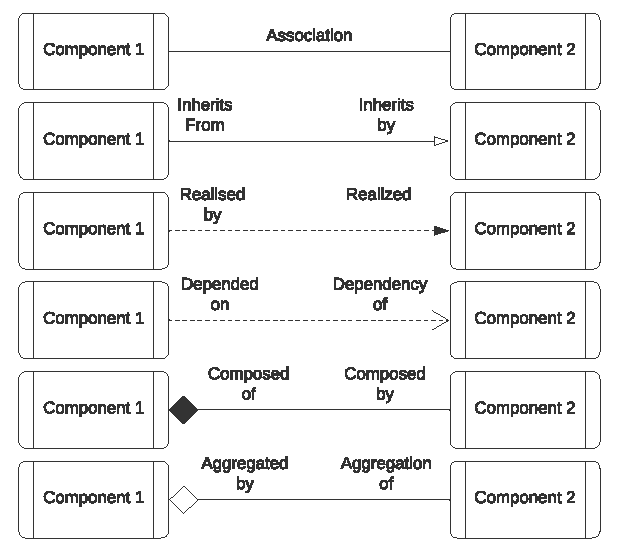
\includegraphics[width=0.5\textwidth]{figures/legenda.pdf}
  \caption[UML Notation used]{UML notation}
  \label{fi:class_diagram_relationship_notation}
\end{figure}